% Written by Jabari Dash

\documentclass{article}

\usepackage{graphicx}
\usepackage{fancyhdr}
\usepackage{enumitem}
\usepackage{caption}
\usepackage{float}
\pagestyle{fancy}

\begin{document}
	\begin{titlepage}
		\begin{center}
			\line(1,0){340}\\
			[0.25in]
			\huge\bfseries Temperature Data Aggregation in Bliss Hall at SUNY New Paltz\\
			[2mm]
			\line(1,0){340}\\
			[1.1cm]
			\textsc{\Large Written by: Jabari Dash\\ May 9, 2016}\\
			[1cm]
			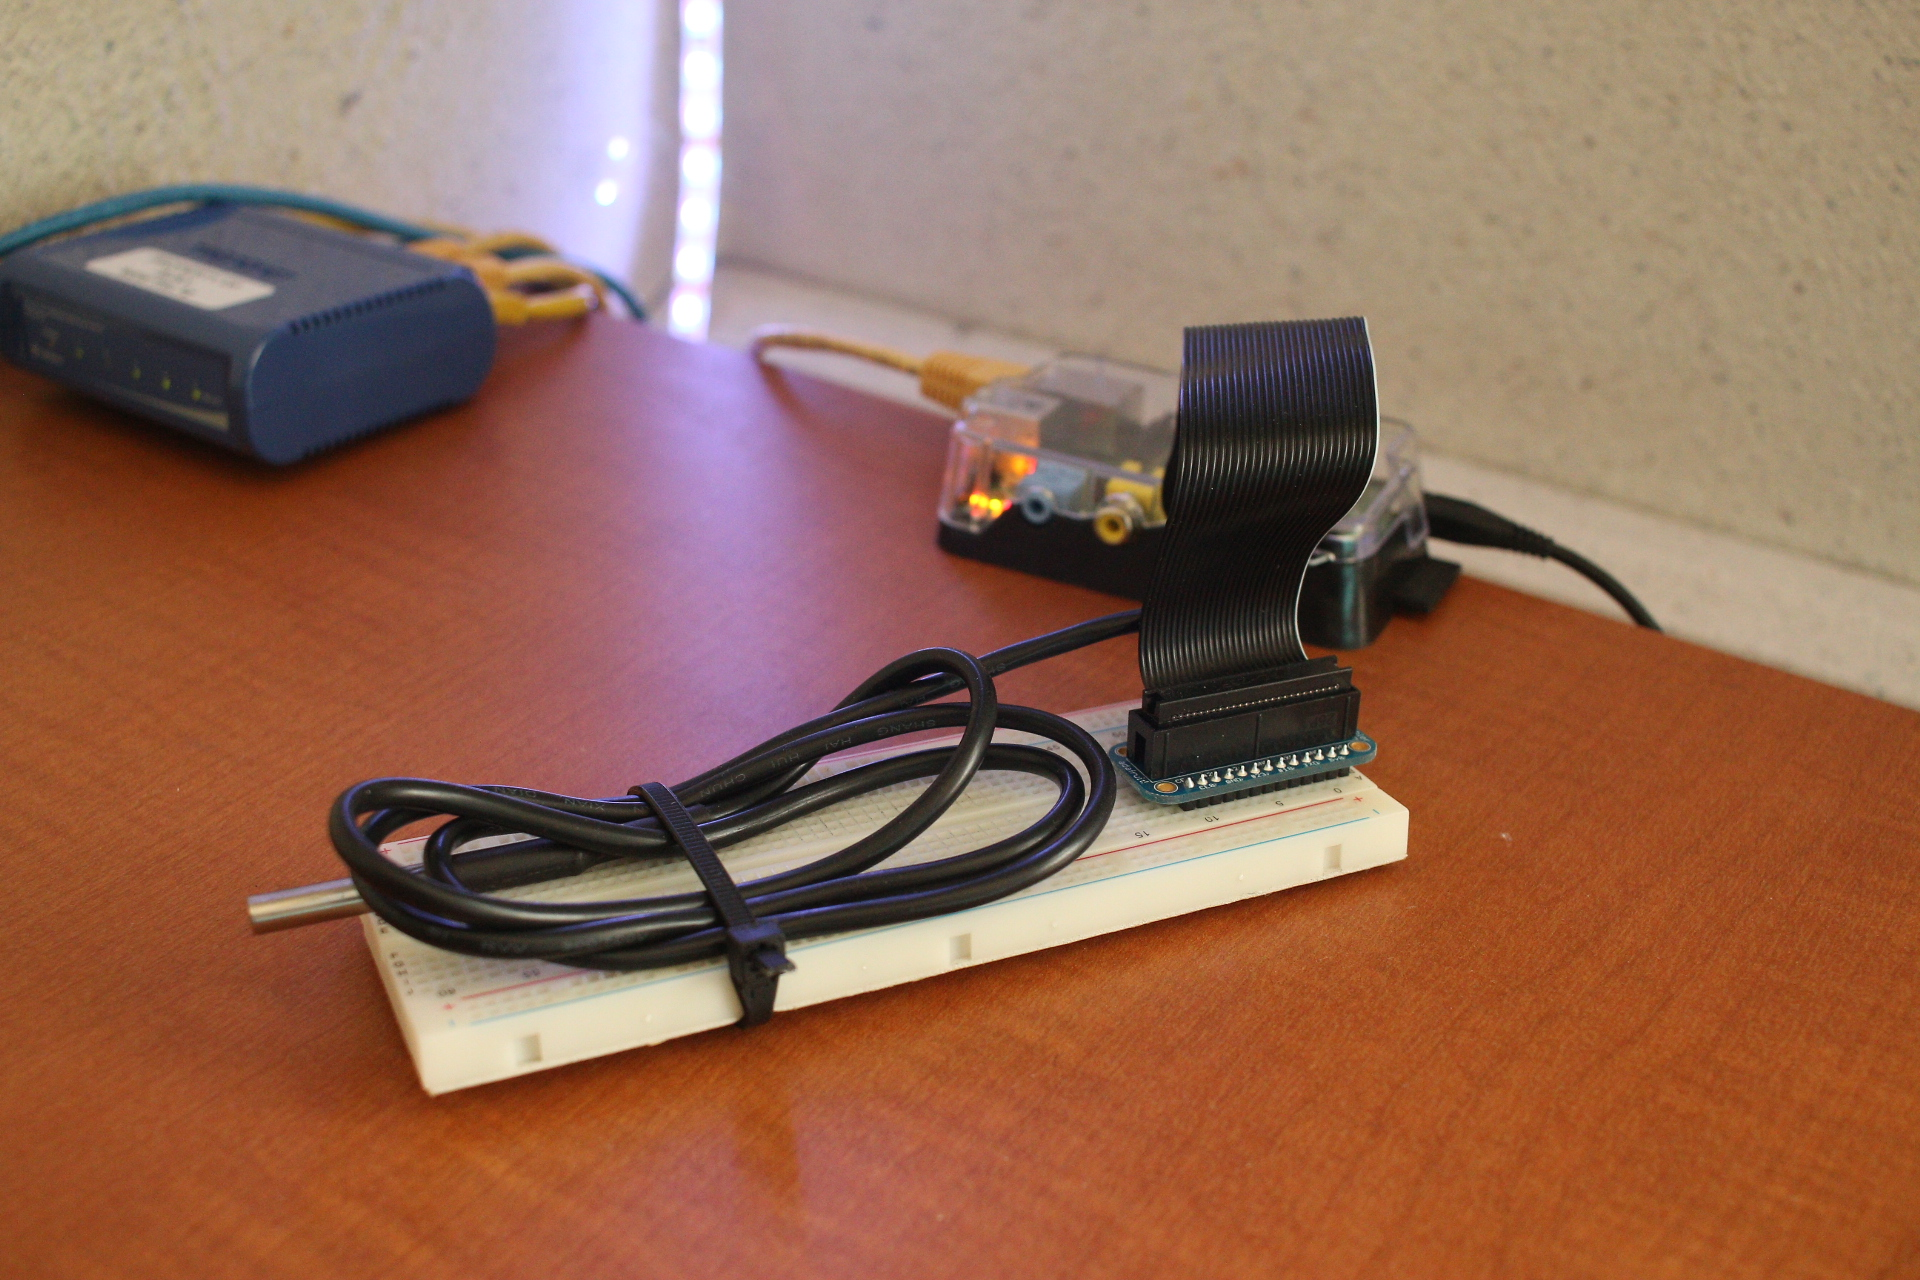
\includegraphics[scale=.15]{rpi.jpg}\\
			[1cm]
		\end{center}
		
		\begin{flushright}
			\textsc{\Large Brendan Lowe\\
				Cesar Done\\
				Heidi Fritz\\
				Jabari Dash\\
				Roberto Milanese\\
				Victoria Bottali\\}
		\end{flushright}
	\end{titlepage}
	
%====================================================================================================================================
	\tableofcontents
%====================================================================================================================================
	
	\newpage	
	\section{Introduction}\label{sec:intro}
		This report documents the process that several students in Dr. Chirakkal Easwaran's Spring 2016
		Embedded Linux class took to complete their final class project. The course is designed to introduce students to 
		the fundamentals of Linux programming - particularly embedded Linux. Dr. Easwaran's course is oriented around the Raspberry Pi
		and the Raspbian (Debian) Linux distribution to give students this fundamental practice. Students throughout the 	
		course learn basic terminal commands, how to read temperature sensors, how write to a SQLite3 database, and more. Midway 
		through the semester, students are separated into groups, and assigned a final project. Students Brendan Lowe, Cesar 
		Done, Heidi Fritz, Jabari Dash, Roberto Milanese, and Victoria Bottali were tasked with collecting 
		temperature data throughout Bliss Hall at the SUNY New Paltz campus and representing it graphically
		for later analysis by the Sustainability Office.                                                                                                                                                                                                                                                                                                                                                                                                                                                                                                                                                                                                                                                                                                                                                                                                                                                                                                                                                                                                                                                                                                                                                                                                                                                                                                                                                                                                                                                                                                                                                                                                                                                                                                                                                                                                                                                                                                                                                                                                                                                                                                                                                                                                                                                                                                                                                                                                                                                                                                                                                                                                                                                                                                                                                                                                                                                                                                                                                                                                                                                                                                                                                                                                                                                                                                                                                                                                                                                                                                                                                                                                                                                                                                                                                                                                                                                                                                                                                                                                                                                                                                                               
		
		\begin{figure} [H]
				\begin{center}
					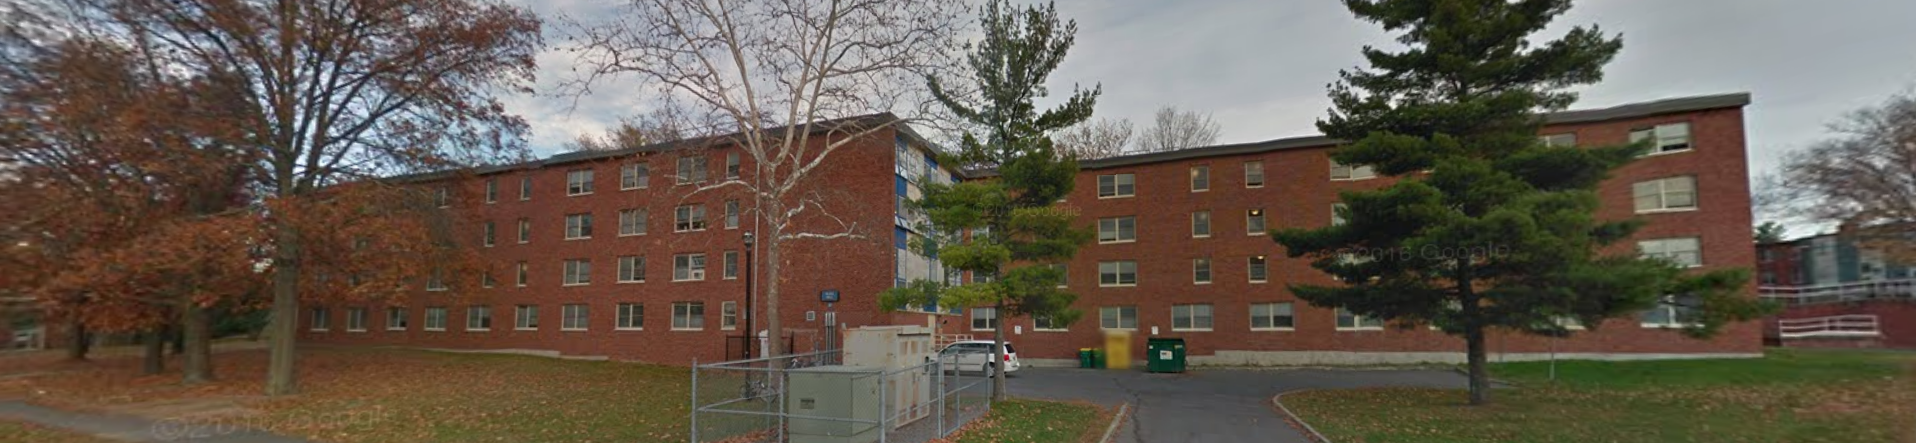
\includegraphics[scale=.3]{bliss.png}
						\captionsetup{labelformat=empty}
						\caption{Google Maps screen-shot of rear of Bliss}
				\end{center}
			\end{figure}
		
%====================================================================================================================================
		
	\newpage
	\section{Individual Student Responsibilities}\label{sec:responsibilities}
		\begin{minipage}{0.45\textwidth}
			\begin{itemize}[label={}]
  				\item
  					\begin{figure}[H]
  						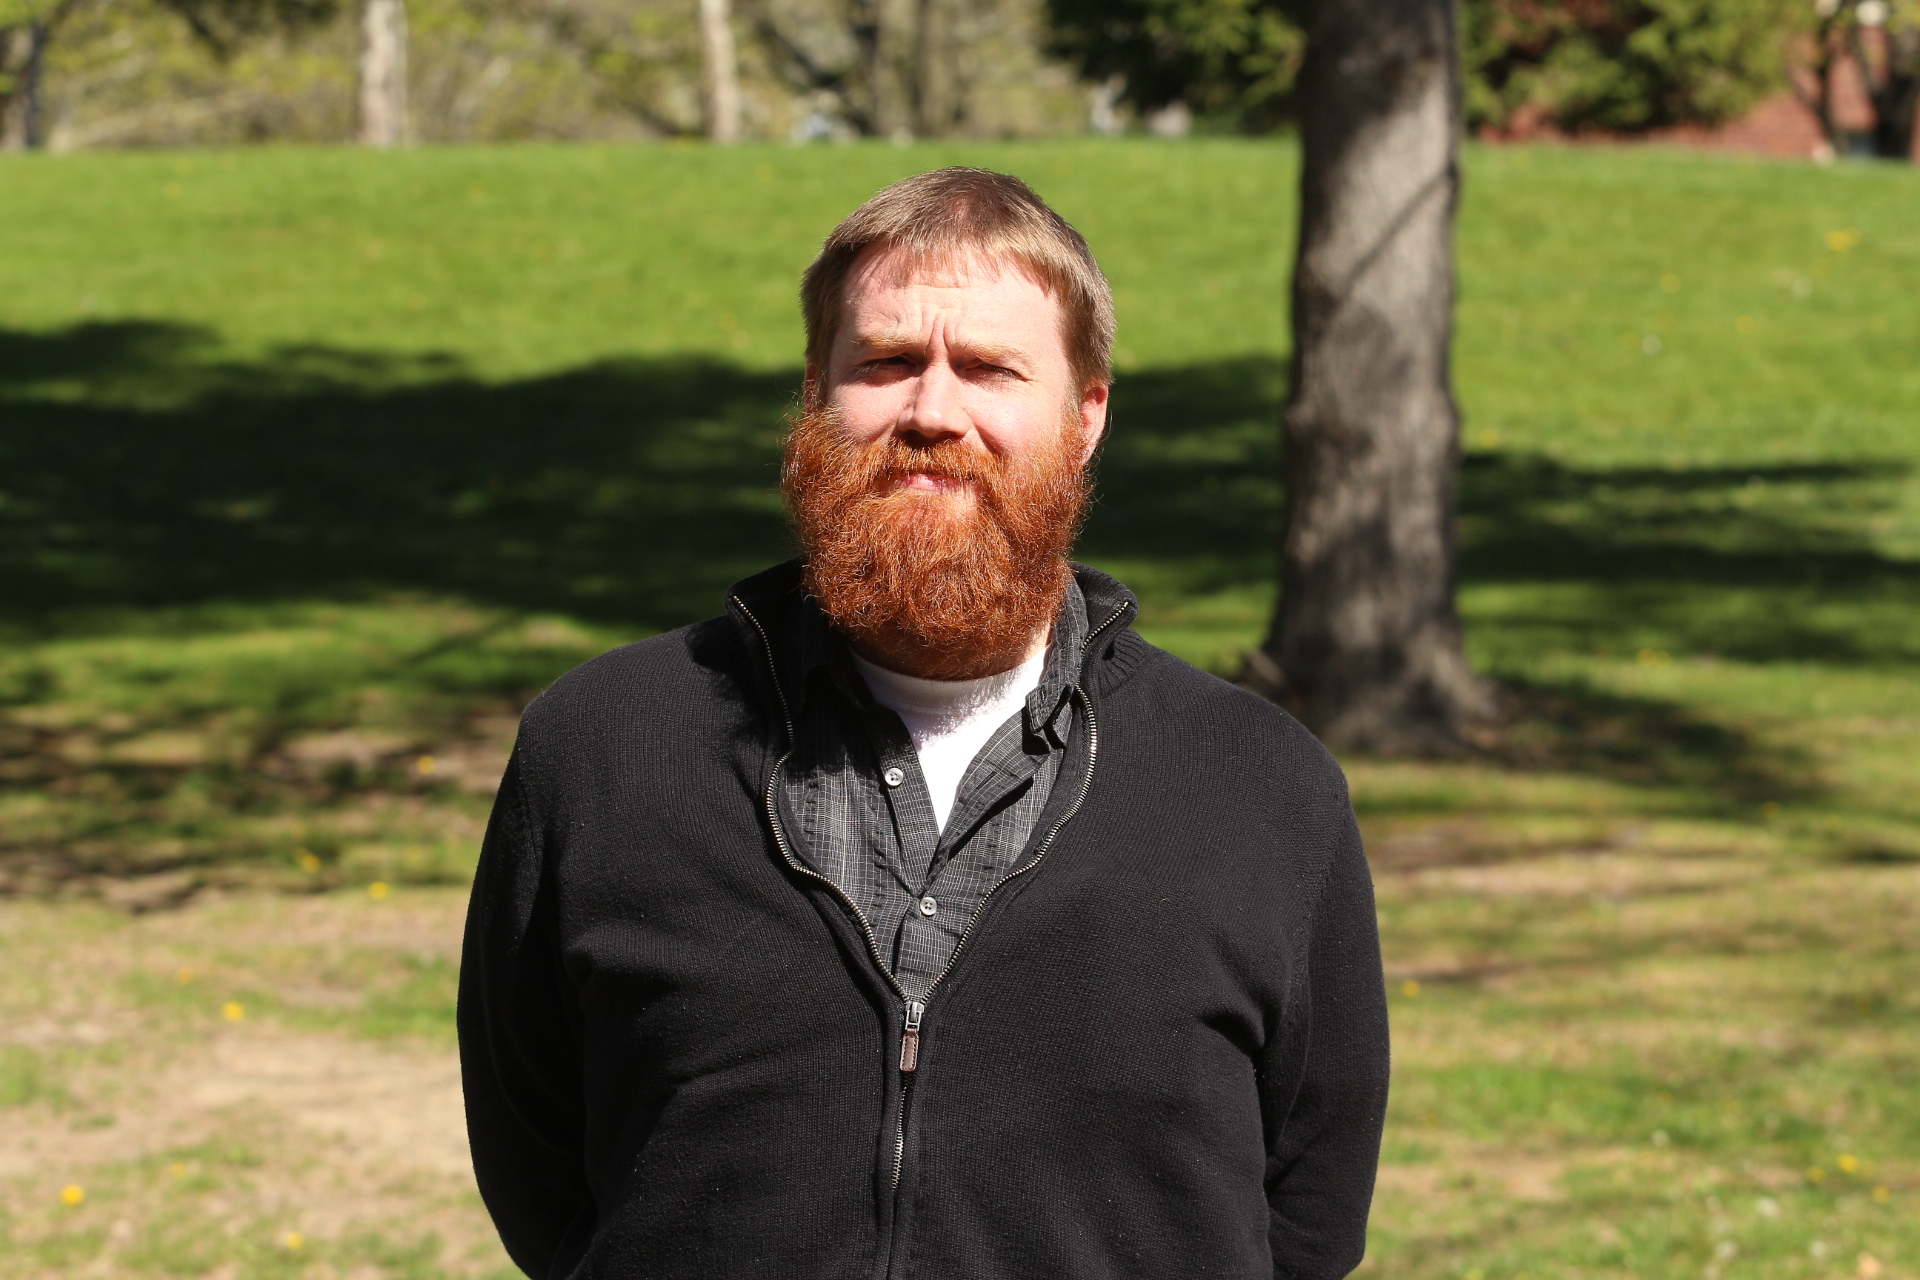
\includegraphics[scale=.07]{brendan.jpg}\\
  							\captionsetup{labelformat=empty}
  							\caption{Brendan handled server-side programming, networking, deployment}
  					\end{figure}
  				\item
  					\begin{figure}[H]
  						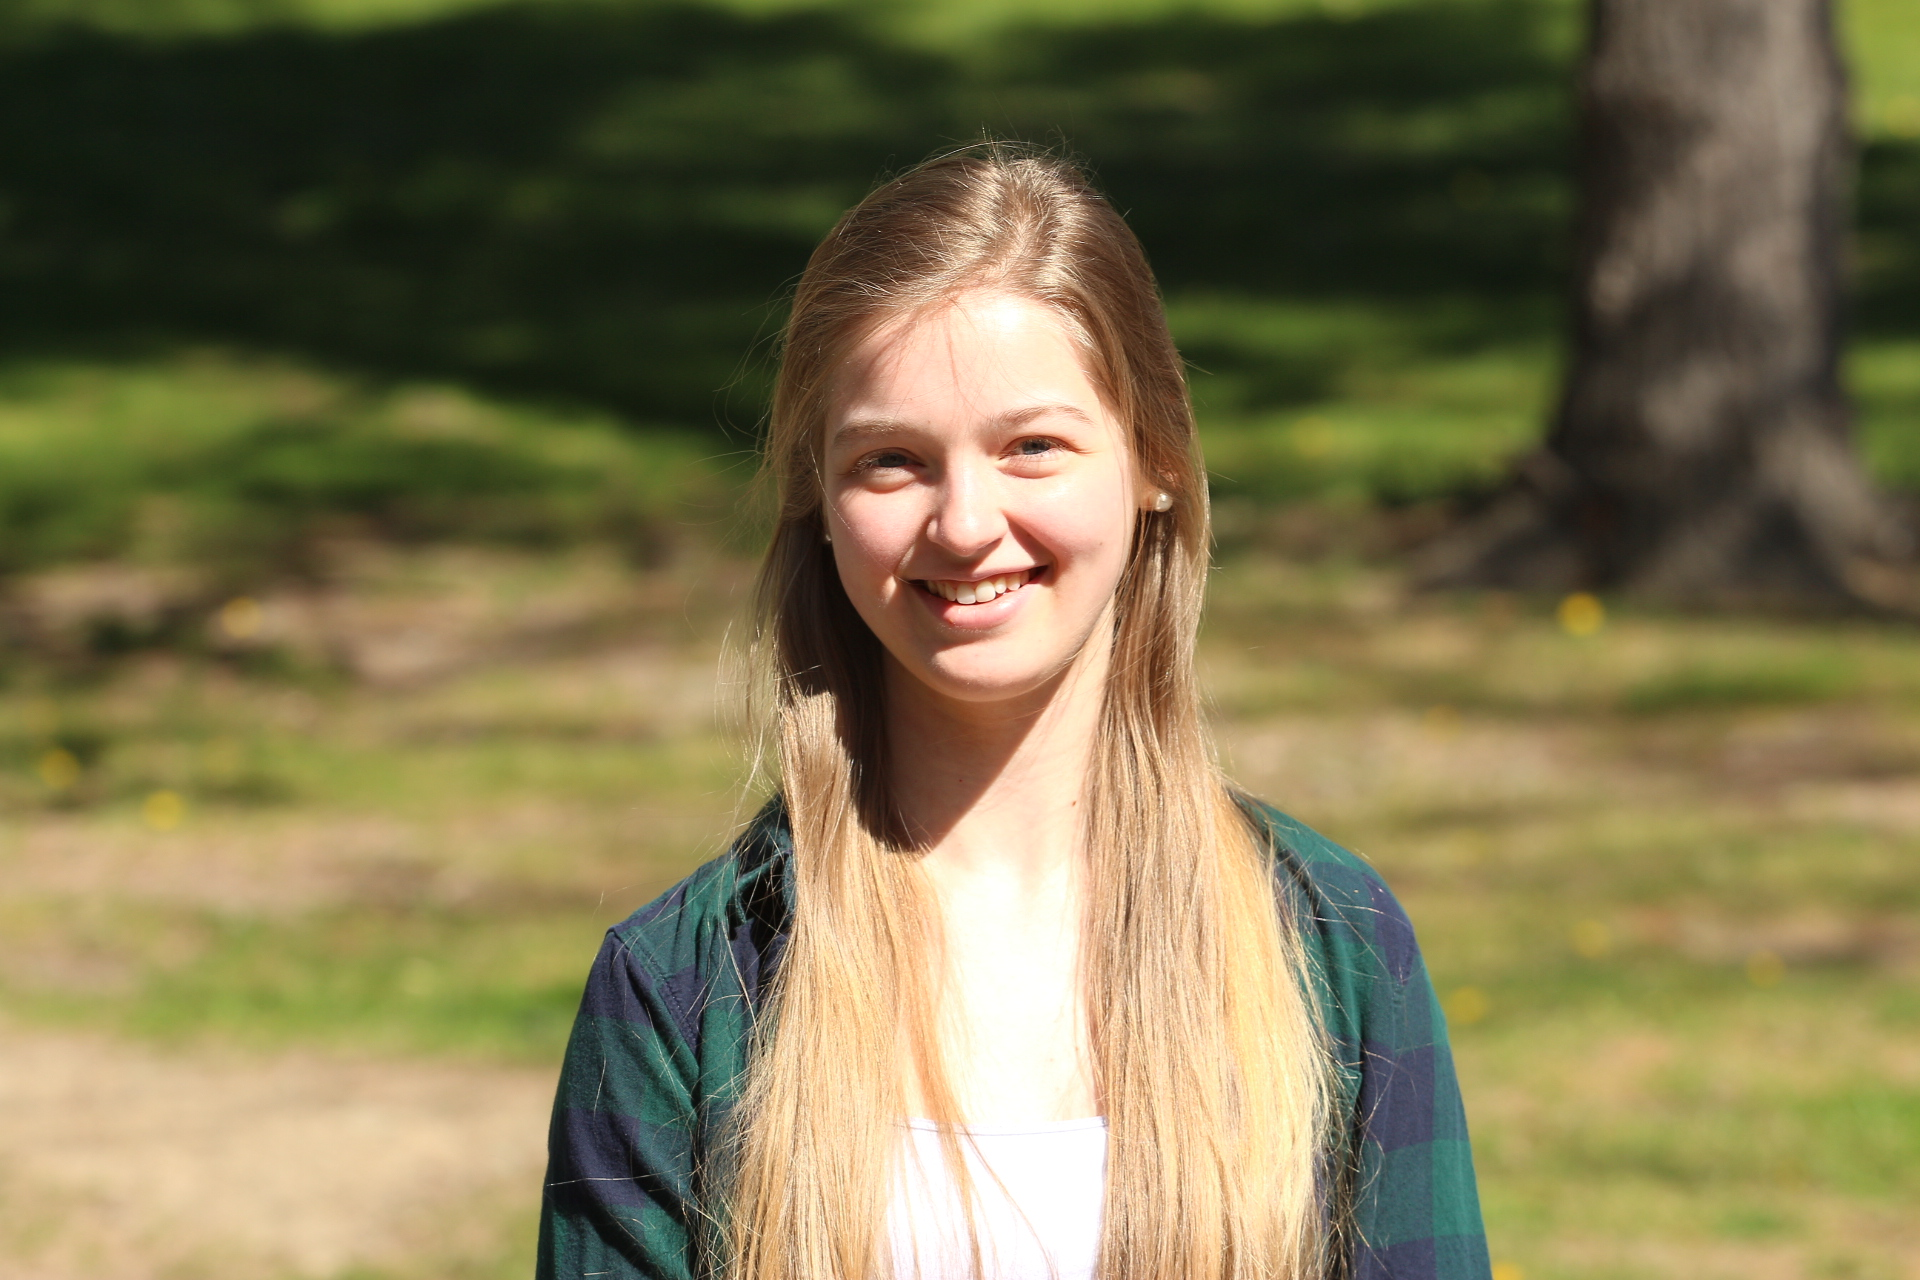
\includegraphics[scale=.07]{heidi.jpg}\\
  							\captionsetup{labelformat=empty}
  							\caption{Heidi handled  client-side programming, front-end programming
  										}
  					\end{figure}
  				\item
  					\begin{figure}[H]
  						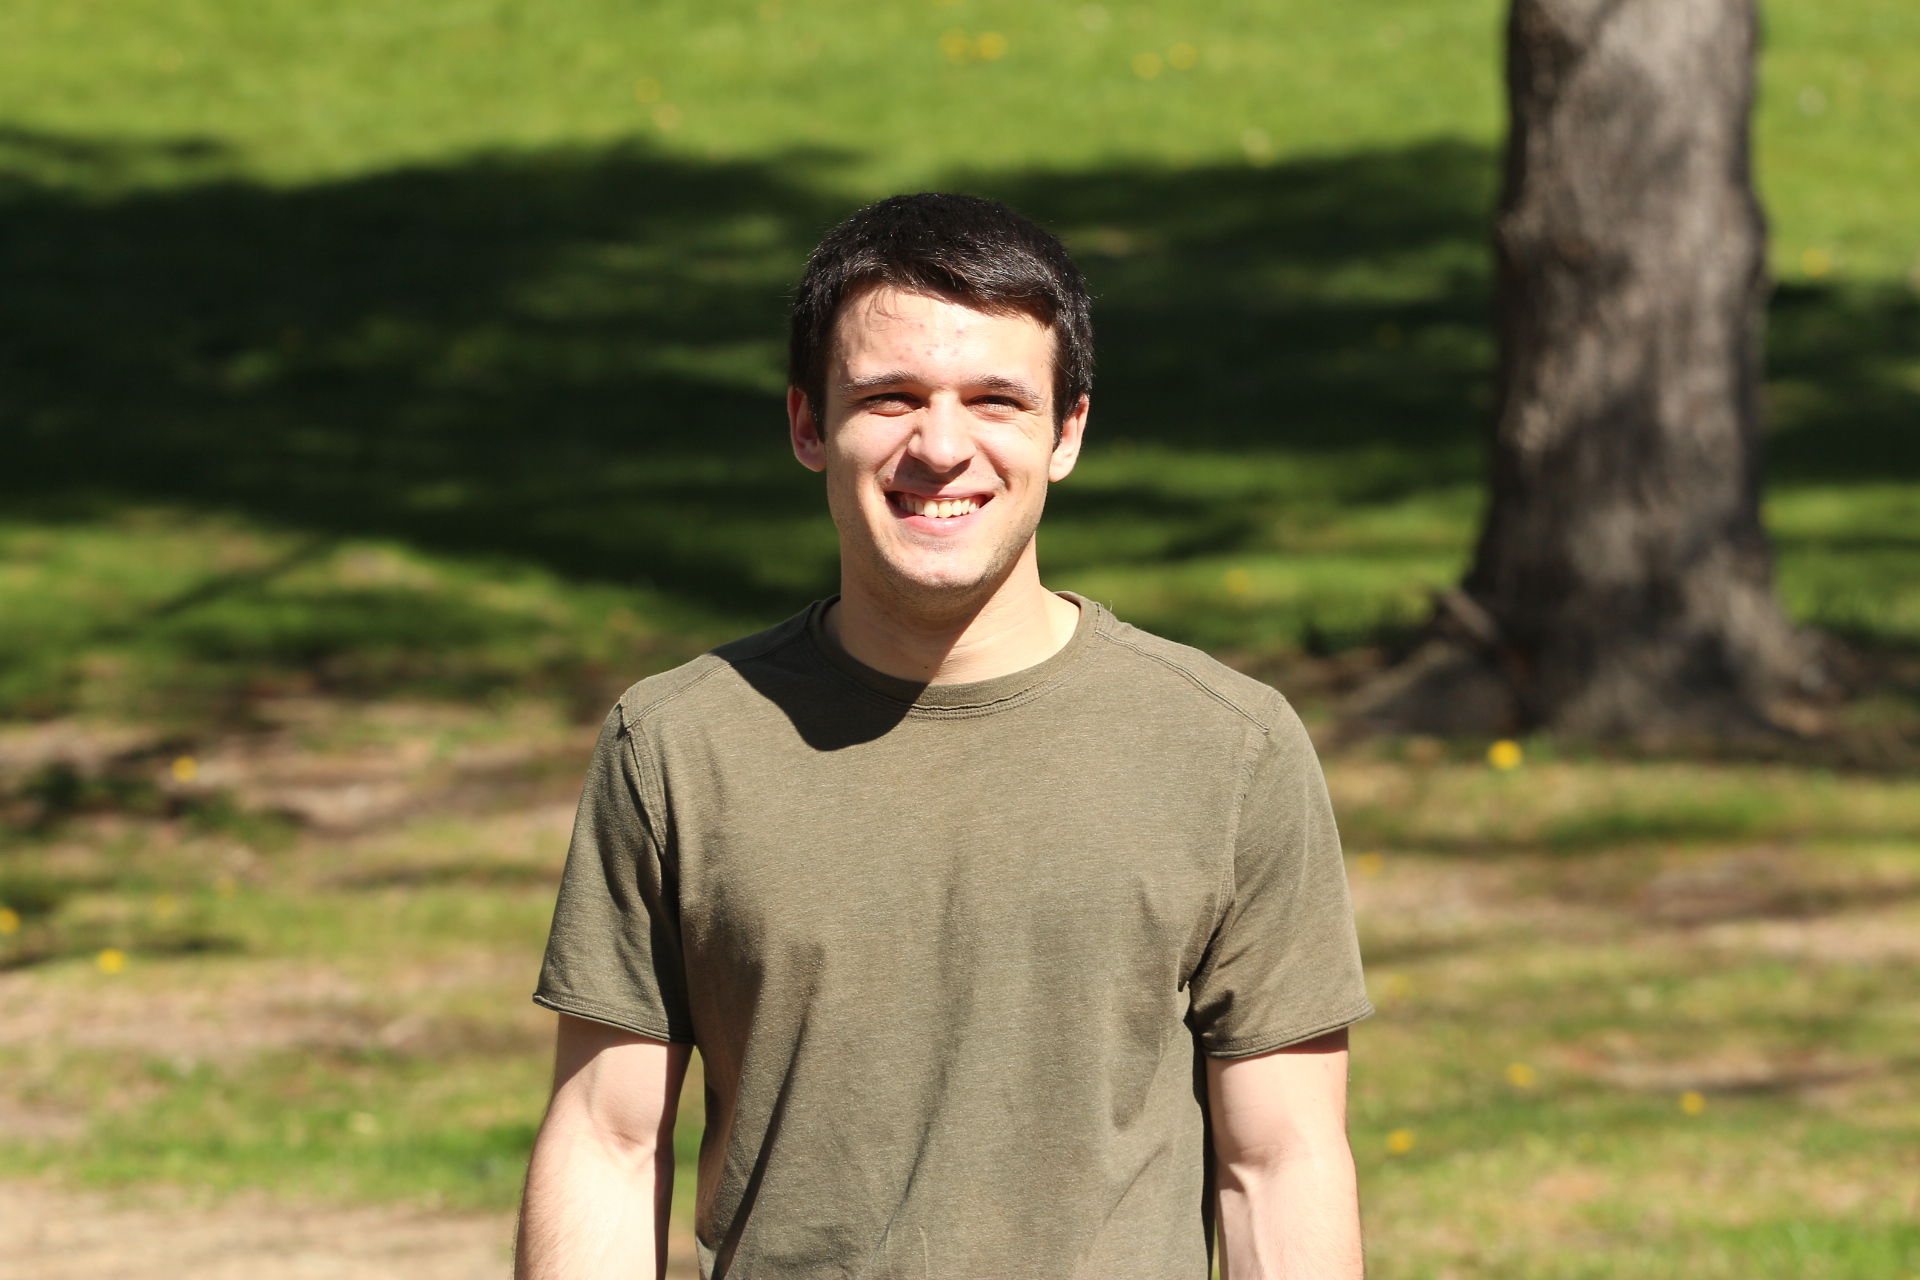
\includegraphics[scale=.07]{roberto.jpg}\\
  							\captionsetup{labelformat=empty}
  							\caption{Roberto handled front-end programming, GUI design}
  					\end{figure}
			\end{itemize}
		\end{minipage}
		\hfill
		\begin{minipage}{0.45\textwidth}
			\begin{itemize}[label={}]
				\item
  					\begin{figure}[H]
  						
\includegraphics[scale=.07]{cesar.jpg}\\
  							\captionsetup{labelformat=empty}
  							\caption{Cesar handled front-end programming, GUI design}
  					\end{figure}
  				\item
  					\begin{figure}[H]
  						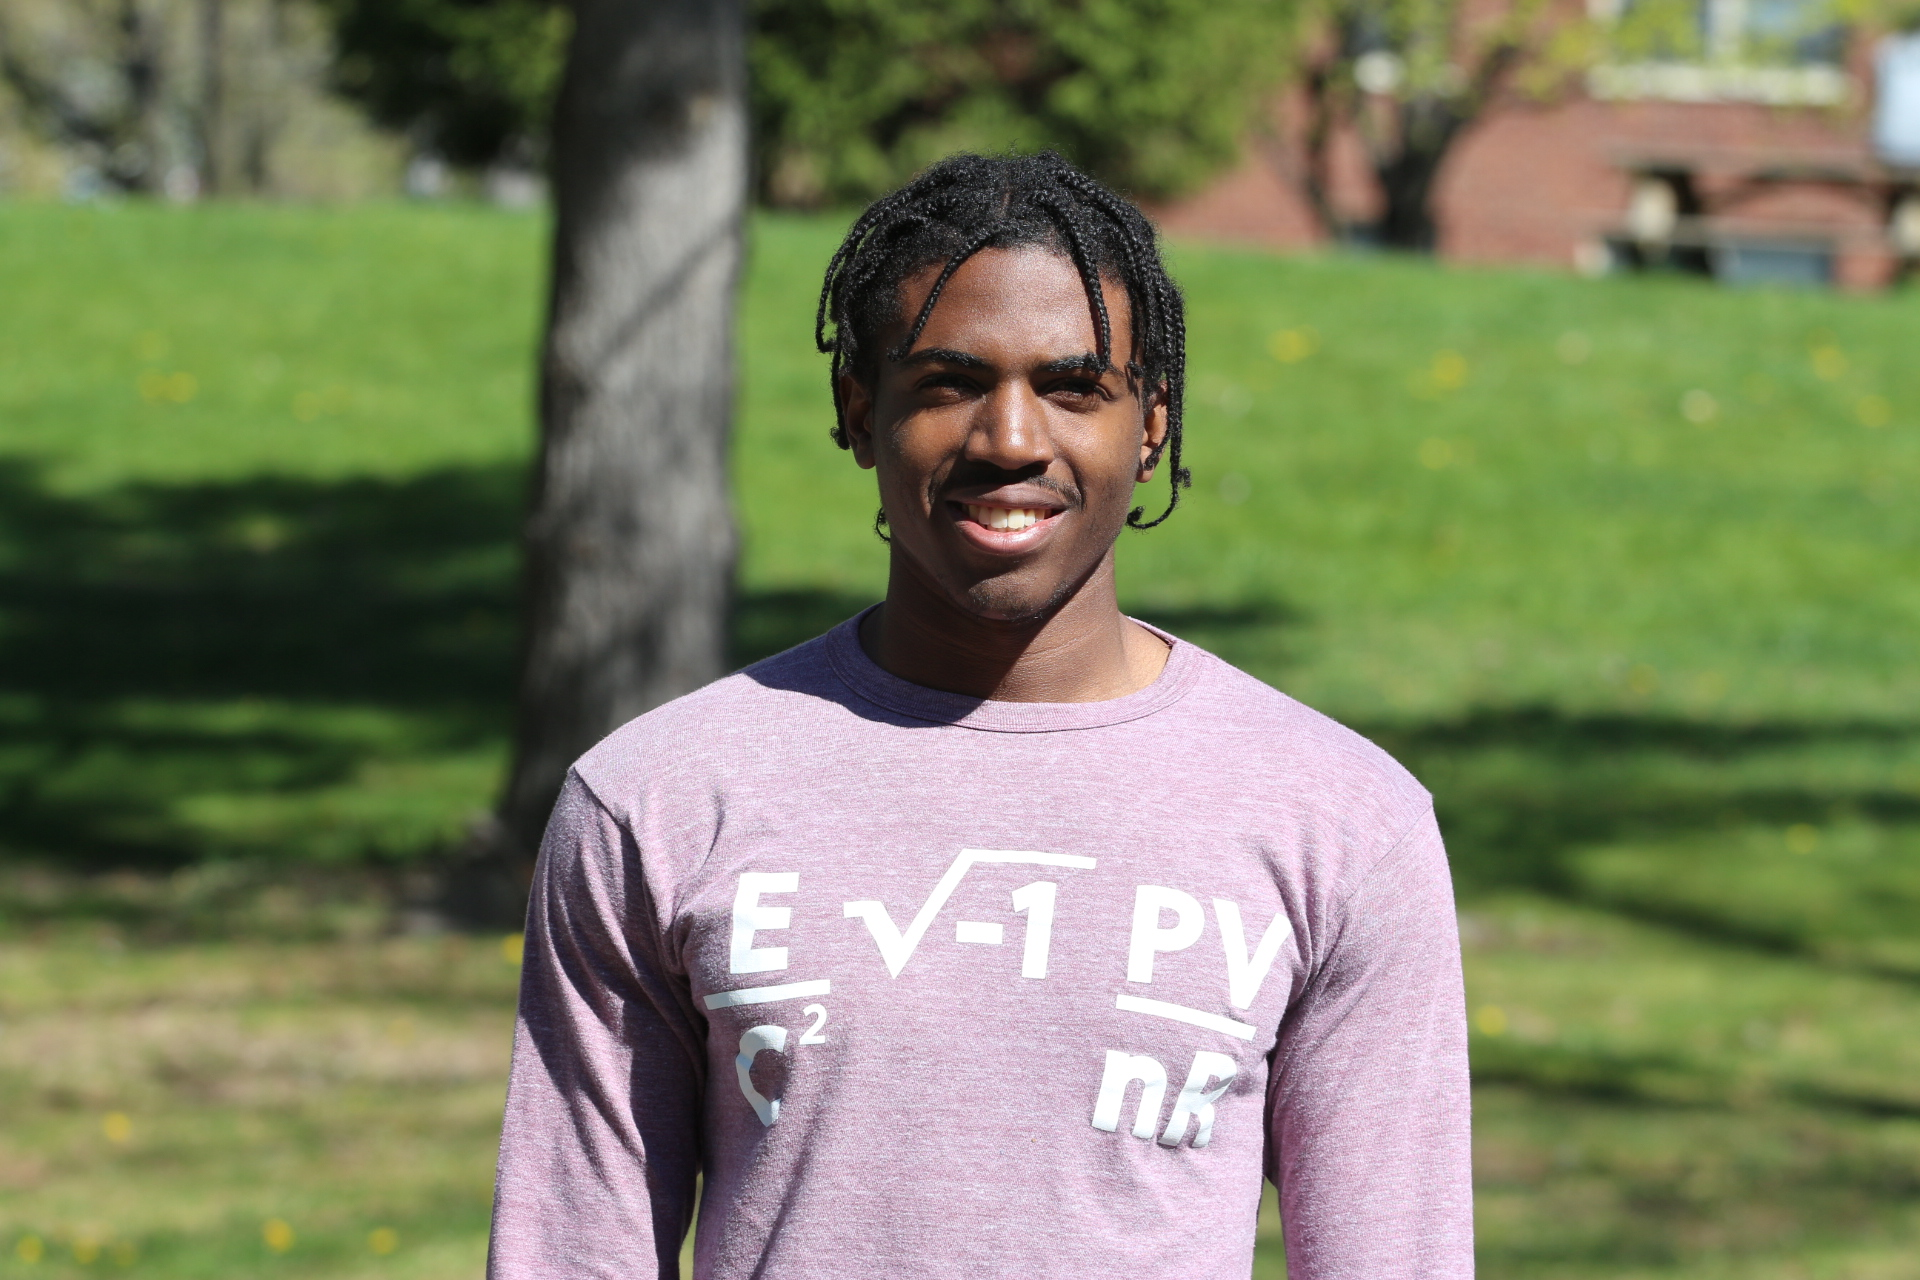
\includegraphics[scale=.07]{jabari.jpg}\\
  							\captionsetup{labelformat=empty}
  							\caption{Jabari handled documentation, logistics, GUI design}
  					\end{figure}
  				\item
  					\begin{figure}[H]
  						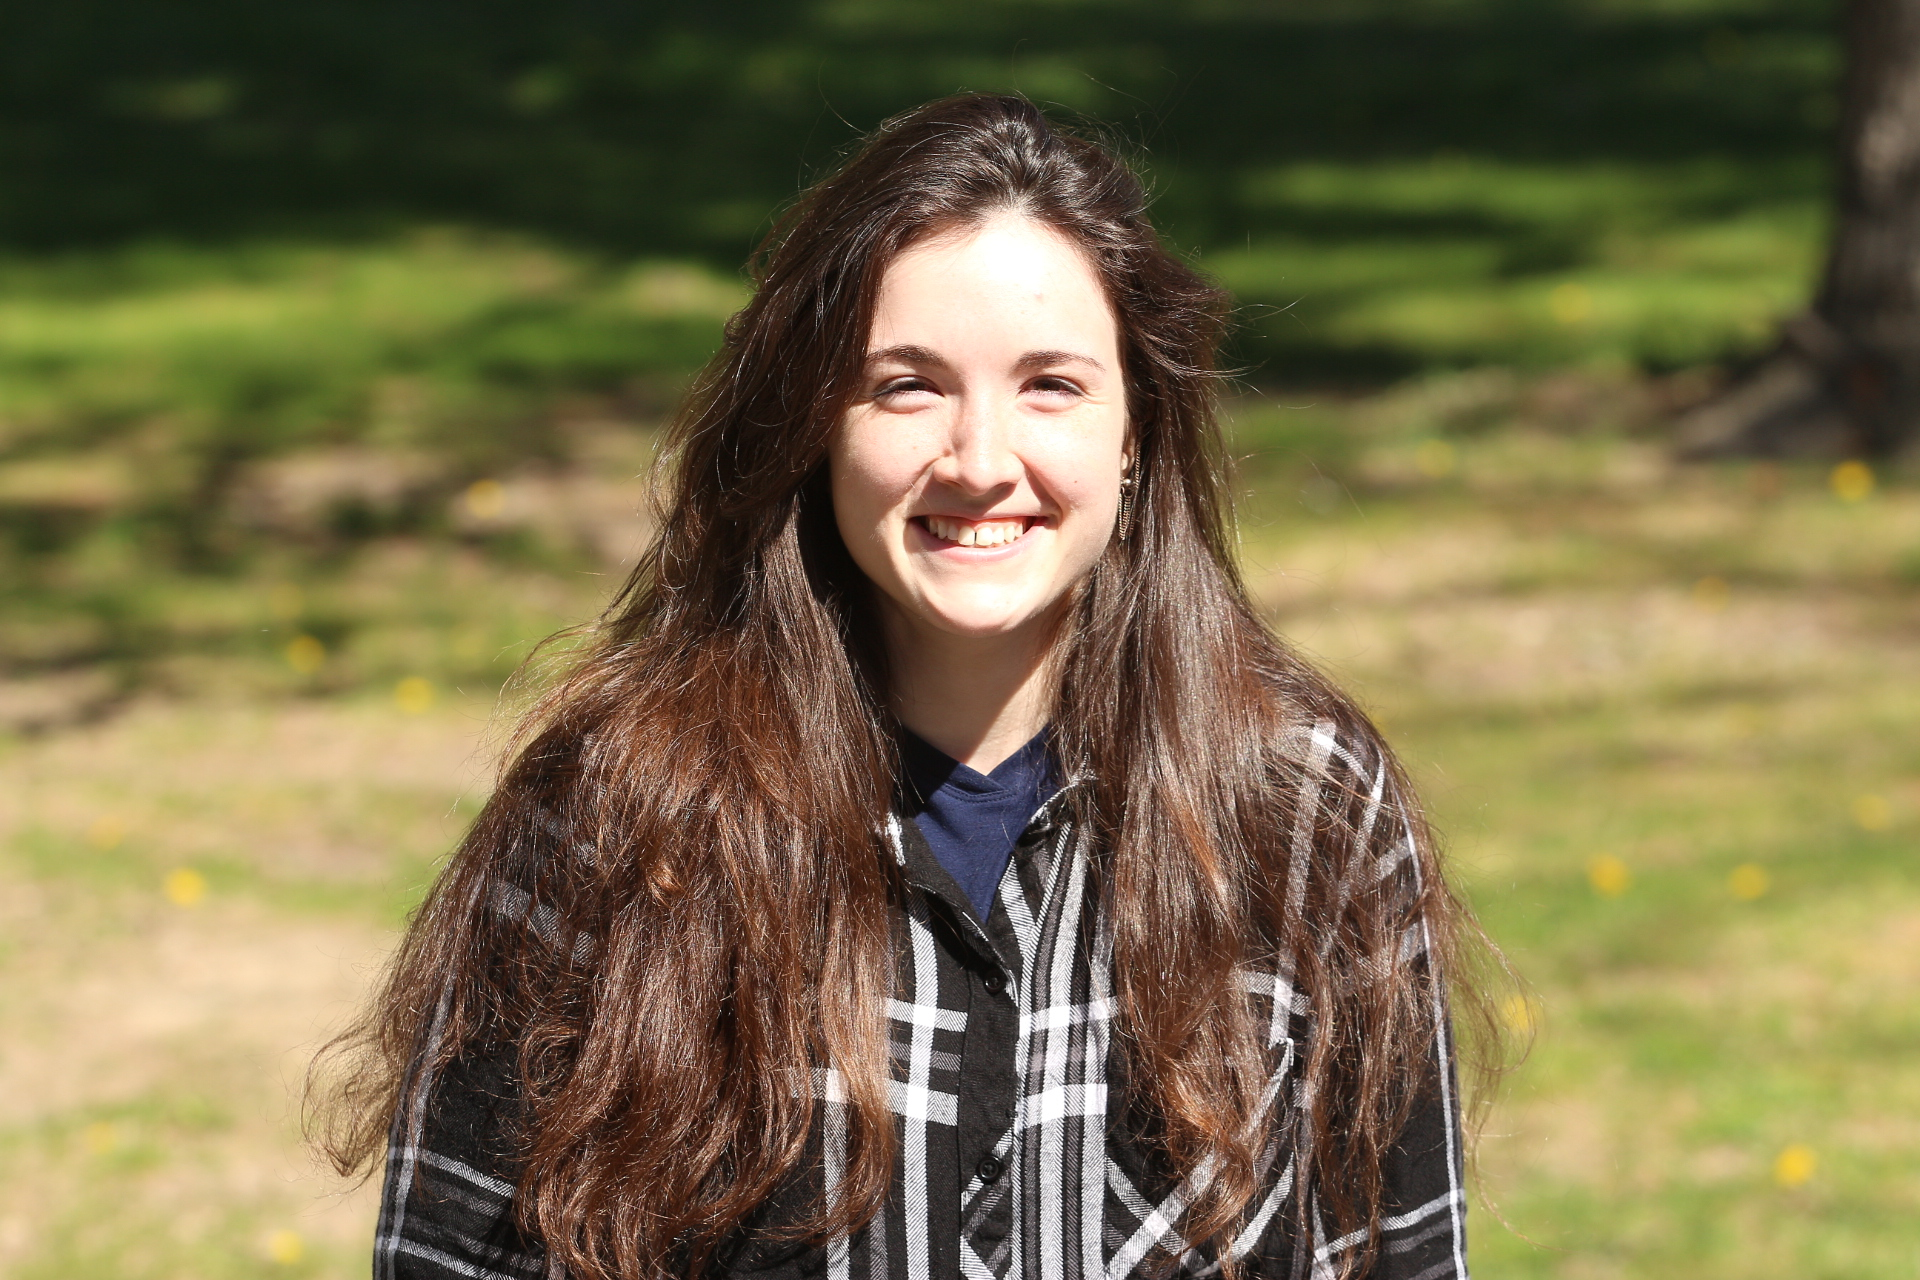
\includegraphics[scale=.07]{victoria.jpg}\\
  							\captionsetup{labelformat=empty}
  							\caption {Victoria handled client-side programming}
  					\end{figure}
			\end{itemize}
		\end{minipage}%
		
%====================================================================================================================================
	
	\newpage
	\section{Project Goals}\label{sec:goals}
		\subsection{Student Learning Outcome Goals}
			For this project students will be provided with first hand experience with software engineering. Being a Software
			Engineer / Developer is different than simply being a Coder or Programmer. A Programmer is someone who knows a set 
			of programming languages, and knows how to write programs as assigned in those languages - the same for a coder. 
			A Software Developer differs in that they analyze a problem, gather a team, and design and implement a solution. 
			The goal of this project is just that. The task of this project is to familiarize students with processes
			and resources that Software Engineers use when creating solutions.
			
			For this given project, students will use resources such as GitHub as a repository for their code. Using GitHub will
			give students the opportunity to work collaboratively, stage, and commit code. They will write software using 
			Python, JavaScript, PHP, SQLite3, MySQL, HTML, and more. They will also obtain some of the soft skills required such
			as team work, communication, and basic negotiation skills (in terms of decision making).
		\subsection{Project Output Goals}
			To have several weeks worth of temperature data on Bliss Hall accessible in a user friendly web page that the
			Sustainability Officer will be able to view and later analyze.\\	
		
		\begin{figure}[H]
  			\begin{center}	
				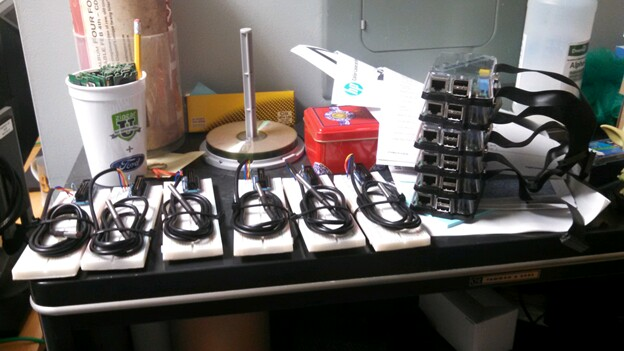
\includegraphics[scale=.5]{pre_deployment.jpg}
			\end{center}
  				\captionsetup{labelformat=empty}
  				\caption{6 Raspberry Pis at the pre-deployment stage}
  		\end{figure}			
			
%====================================================================================================================================
		
	\newpage	
	\section{Materials \& Programming Languages}\label{sec:materials}
		\subsection{Hardware}
			\begin{itemize}
				\item Raspberry Pi Single Board Computer (8)
				\item Adafruit Raspberry Pi Enclosure(8)
				\item MicroUSB + Wall Adapter Kit (8)
				\item 4GB + SD Card (8)
				\item Cobbler Cable + Pi Header Kit (8)
				\item DS18B20 Digital Temperature Sensor (8)
				\item Breadboards (8)
				\item 4.7k Ohm Resistor (8)
				\item Ethernet Cables (9)
				\item Networking Switch (1)
				\item Wire Tie (8)
				\item Duct Tape
			\end{itemize}
			
		\subsection{Software}
			\subsubsection{Client-Side Programming}
				\begin{itemize}
					\item Crontab
					\item HTML
					\item JavaScript
					\item Python
					\item SQLite3						
				\end{itemize}	
			\subsubsection{Server-Side Programming}
				\begin{itemize}
					\item MySQL
					\item PHP									
				\end{itemize}
			\subsubsection{Documentation}
				\begin{itemize}			
					\item GitHub
					\item LATEX
				\end{itemize}
		
%====================================================================================================================================
			
	\newpage
	\section{Implementation}\label{sec:implementation}
	
		Students distributed several internet connected Raspberry Pi computers throughout Bliss Hall in residents' rooms
		where each Pi periodically (every 10 minutes) reads the current ambient temperature in the room and writes it to a local database. A 
		Linux Apache MySQL and PHP (LAMP) server running on SUNY New Paltz servers periodically performs a pull request on
		each Pi, and compiles all of the temperature data in a MySQL database. This data can then be viewed graphically on a 
		live website - hosted by school servers.	
		
		The website, and the project overall implements the Model View Controller (MVC) design pattern. This means that the Model (the data),
		the View (GUI), and the controller (server) are all coded separately from each other. 
		
		\begin{figure} [H]
			\begin{center}
				\includegraphics[scale=.3]{../graphs/TempSensorProgramFlowOfEvents.png}
			\end{center}
			\captionsetup{labelformat=empty}
			\caption{Overall flow of the temperature sensor project}
		\end{figure}
		
%------------------------------------------------------------------------------------------------------------------------------------
			
	\newpage
			
		\subsection{Temperature Sensor Setup}	
			The temperature sensor is connected to the Raspberry Pi's General Purpose Input Output (GPIO) pins via breadboard, 
			and the 24-pin cobbler cable. The DS18B20 has three cables: ground (GND), 3.0v - 5.0v power line, and a data line. 
			We connect the GND to the GND pin on the Raspberry Pi, the power line to the 3.3v rail, and the data line to GPIO \#4.
		 	We then set up a pull-up resistor that connects the data line (pin 4) to the 3.3v line. Temperature sensors were set
		 	up by Brendan and Jabari, and deployed by Brendan.
							
				\begin{figure}[H]
  					\begin{center}	
						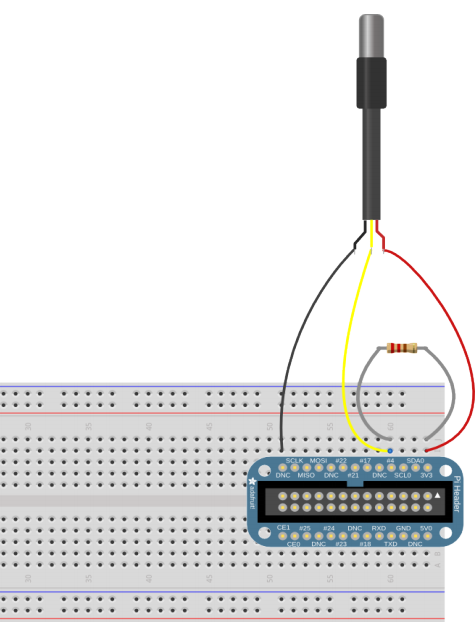
\includegraphics[scale=.8]{breadboard.png}\\
					\end{center}
  						\captionsetup{labelformat=empty}
  						\caption{DS18B20 Digital Temperature Sensor connected to the breadboard using a  4.7k pull-up resistor}
  				\end{figure}	
						
%------------------------------------------------------------------------------------------------------------------------------------  	
  	
  	\newpage	
  		\subsection{Model}		
  			In the MVC design pattern, the Model handles how data is stored. For this project, a combination of SQLit3, MySQL, PHP,
  			and Python were used to implement the Model - both on the Raspberry Pi and on the LAMP server.

			\subsubsection{Programming the Raspberry Pi using Python Scripts}
				Each Pi has 3 Python scripts that allow the Pi to collect data, convert it to JavaScript Object
				Notation (JSON) format, and return the JSON to the LAMP server. The temperature data is stored locally
				in the SQLite3 database. This information is then copied, and sent to the LAMP server. This is for the 
				purpose of redundancy. For example, in the event that internet connection is lost between the client and
				the server, as soon as the connection is restored, all of the data collected offline can sent to the server.

				\begin{itemize}
					\item {\bfseries tempLog.py}: Creates a Cronjob (scheduled task) the first time tempLog.py executes. The Cronjob 
									  executes tempLog.py every 10 minutes. The script reads the ambient temperature
									  in Celcius and writes it to a SQLite3 database file called climate\_info.db. tempLog.py was
									  written by Heidi.
						\begin{figure}[H]				
							\begin{center}
								\includegraphics[scale=.35]{../graphs/tempLog.png}\\
							\end{center}
							\captionsetup{labelformat=empty}
							\caption{tempLog.py program flow}
						\end{figure}
						
					\item {\bfseries index.py}: When passed a given start and stop date, index.py sets up a Flask server on the Pi and 
									converts the data from the SQLite database into JSON objects. The JSON is put onto the Flask server in
									preparation to be sent to the LAMP server. index.py was written by Brendan.
					\item {\bfseries json\_push.py}: Is responsible for communicating with the LAMP server. json\_push sends an HTTP GET request
													 to the LAMP server for the last date that the MySQL database has for that Pi. This script
													 then calls index.py to get and send all data after that date as a HTTP POST back to the server.
													 json\_push.py was written by Brendan.
				\end{itemize}
				
			\subsubsection{SQLite3 Database Schema (on Raspberry Pi)}	
				Each Pi has a SQLite3 database file called climate\_info.db that stores all of the temperature data, and device specific information
				for identification purposes.
				
				\begin{center}
					\includegraphics[scale=.7]{../graphs/sqlite3_schema.png}
				\end{center}
			
			\subsubsection{MySQL Database Schema (on LAMP Server)}
				\begin{figure}[H]
					\begin{center}
						\includegraphics[scale=.6]{../graphs/MySQL.png}
					\end{center}	
				\end{figure}
			
		\subsection{View}
			The View is what the user actually sees, and interacts with. 
			For this project, students were asked to implement two different views of the same data.		
		
			\subsubsection{Graphical User Interface (GUI) by Group A}
				GUI A is written by Heidi and Jabari. It is written in HTML, JavaScript, and PHP, and implements Google Charts API to graph data.
				
				\begin{figure}[H]
					\begin{center}
						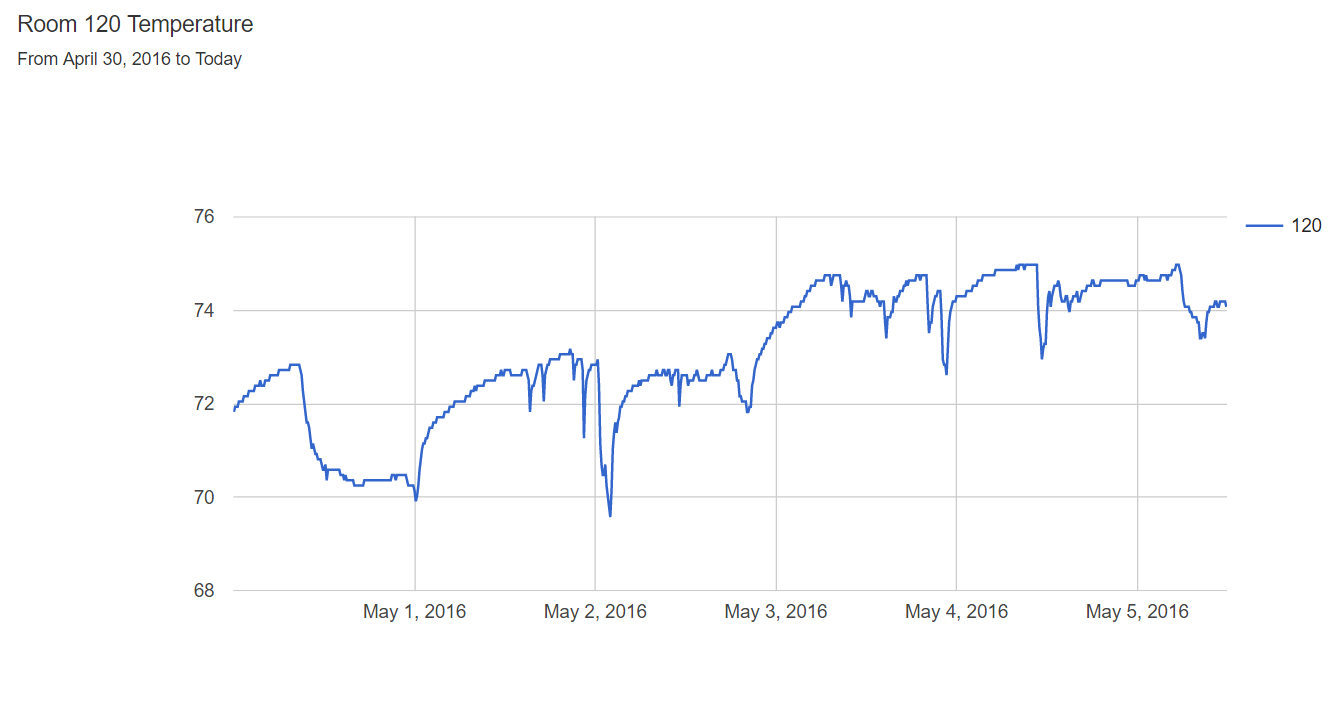
\includegraphics[scale=.4]{TempVersusTime.PNG}			
					\end{center}
					\captionsetup{labelformat=empty}
					\caption{Google Chart's Line Chart used to graph temperature versus time by room}
				\end{figure}				
				
				\begin{figure}[H]
					\begin{center}						
						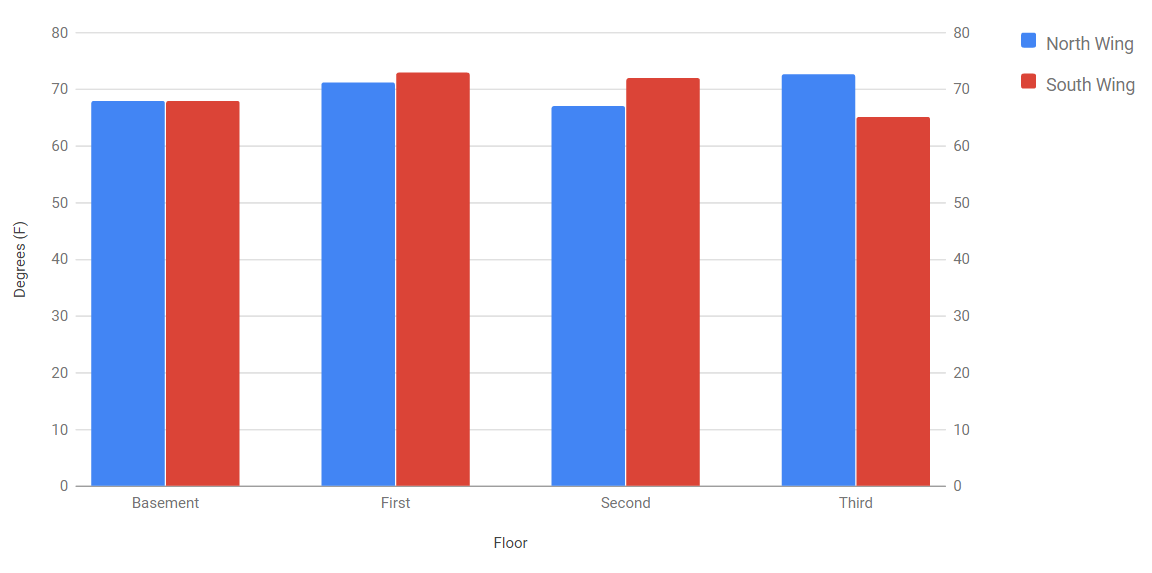
\includegraphics[scale=.5]{averageFloorTemp.PNG}				
					\end{center}
					\captionsetup{labelformat=empty}
					\caption{Google Chart's Bar Chart used to graph average temperature by floor}
				\end{figure}			
			
			\subsubsection{Graphical User Interface (GUI) by Group B}
				GUI B is written by Victoria and Roberto. It is written in HTML, and Python, and implements the Pygal and Flask libraries to graph
				data.
				
				\begin{figure}[H]
					\begin{center}
						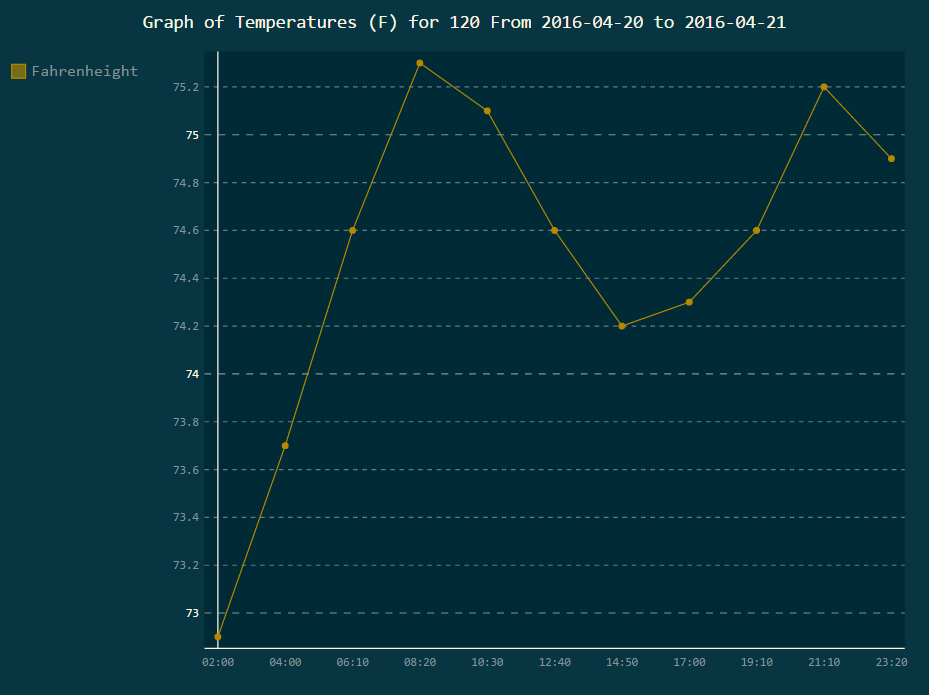
\includegraphics[scale=.48]{../graphs/GUI_B_by_room.PNG}
					\end{center}
					\captionsetup{labelformat=empty}
					\caption{Pygal Python library used to graph temperature versus time by room}
				\end{figure}			
				
				\begin{figure}[H]
					\begin{center}
						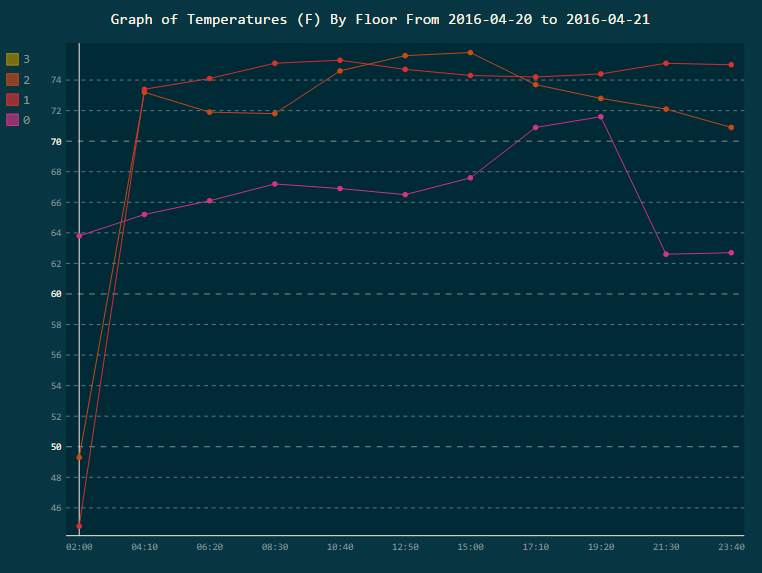
\includegraphics[scale=.58]{../graphs/GUI_B_by_floor.PNG}
					\end{center}
					\captionsetup{labelformat=empty}
					\caption{Pygal Python library used to graph temperature versus time by floor}
				\end{figure}
												
%------------------------------------------------------------------------------------------------------------------------------------
			
	\newpage		
			
		\subsection{Controller}
			The Controller is responsible for getting data back and forth between the Model and the View. In this case, the Controller
			is also responsible for getting data from one element of the Model, to the other. For example, the periodic pull request 
			from the server to each Pi collects the local data from each Pi, and compiles all of the temperature data into one large
			database on the LAMP server.
			
			\begin{center}
				\includegraphics[scale=.7]{tempSensorProgramFlow.png}\\
			\end{center}
					
			\subsubsection{Important PHP Scripts}		
				\begin{itemize}
					\item {\bfseries\ api\textbackslash input.php}: Allows basic interaction between the Raspberry Pi and the LAMP server. Specifically json\_push.py.
														Provides basic point of data collection. This script receives an HTTP GET request from the Pi that 
														request when (via datetime)
														was the last time this (a given Raspberry Pi) has pushed back to the MySQL database. input.php then  
														passes the most recent date back to json\_push.py. The Pi then queries its own database, collects all 
														data after this date, and sends it back in the form of an HTTP POST to input.php. input.php then takes 
														the JSON data and writes it to the MySQL database on the LAMP server.
										  
					\item {\bfseries api\textbackslash climate.php}: Receives HTTP GET (AJAX) requests for temperature data for a given room in the form of a 	 																	 JSON file. 
														 The script can also be provided an optional start and stop date to limit the range of the data that 
														 is returned. If these 2 optional arguments are not provided, the full history for a given room is 
														 provided by default. This file can be used to view a data dump, but is also use in the GUI for 
														 parsing and graphic.
					\item {\bfseries api\textbackslash device.php}: Answers AJAX requests for the list of devices that have entries in the temperature 			 																	database. This is
										 		        in place for future device management - ability to add, remove, and contact individual devices on the 
										 		        project.
					\item {\bfseries device\textbackslash index.php}: Works in conjunction with api/device.php to display the devices on the project.	
					
					\item {\bfseries inc\textbackslash climate.php}: Used for inputting and querying data from the MySQL database.  	
					
					\item {\bfseries inc\textbackslash device.php}: Provides device management features. Currently allows for the ability to add devices to 	 																	the project
														and display specific information about devices.
					
					\item {\bfseries inc\textbackslash main.php}: Provides functions for MySQL database connection, and references for password files. 
													  Also offers array treatment functions (SQL Escape and HTML entity treatment). This prevents
													  SQL inject (injecting commands / queries into others queries). HTML entity treatment prevents special 
													  characters from negatively impacting HTML (being parsed incorrectly).	
				\end{itemize}						
		
%====================================================================================================================================		
	\newpage
	\section{Student Analysis}\label{sec:analysis}
		\subsection{As of April 25, 2016}
			\begin{itemize}
				\item {\bfseries Brendan Lowe}:
				\item {\bfseries Cesar Done}: The project thus far has been running very smoothly. We are lucky to have access to several rooms here on campus as well 
								  as several network settings that students do not regularly have. The Pis have not given us any problems and the actual set 
								  up and maintenance of them have been smooth as well. This project can  become a even bigger, funded project by the school
								   if we manage to provide accurate as well as beneficial data to the school. Also if we can create a simple interface that 
								   school can use to access the data, they would be more inclined to support and provide their services for the project. 
							
				
				\item {\bfseries Heidi Fritz}: This project had simple tasks that we planned out and I took on the back end operations that the raspberry pi would 
				carry out to collect the temperature and humidity data.  To do this I connected my own temperature sensor to a personal pi and wrote 
				python script which consisted of four functions.  A function to get the temperature from the device, log the temperature and time into a 
				SQLite3 database, create a Cronjob to repeat data collection, and a main function to start the process.  One struggle I came across was 
				opening the device file so it would work on every pi.  I imported glob to find the correct path name within the pi.  The python script 
				was easily integrated with the other scripts to work on one pi so we could make copies of the SD card.  In the end, I met the team goals 
				and expectations.
				\item {\bfseries Jabari Dash}: The project so far is going well in that the data is being collected correctly.
									The beginning was challenging in that the group was lost because we were unsure of how to 
									implement this project - particularly the intercommunication between the 
									Raspberry Pis and the server. We wanted to used static IP addresses on the 
									school network, but this was not permitted. Fortunately, Brendan's skill in networking,
									and more importantly, his position as the Networking Manager allowed us to have a subnet
									on the school network, with static IP addresses. This was a "quick and dirty" solution that 
									allowed us to focus more on other elements of the projects, but also reduces the scalability
									and portability of our implementation.
				\item {\bfseries Roberto Milanese}: The project is moving along well. It was harder than expected to get the Pis set up for deployment, and we 													luckily had a group member able to make amendments to the network to help us even further. I look forward 														to beginning GUI/front end development.
				
				\item {\bfseries Victoria Bottali}:	My goal for the end of the project is to have a working Flask app that is able to graph 
										the temperature from the back-end based on different sets of parameters passed via user input. More 				
										specifically, I would like the app to be able to dynamically plot data given a broad spectrum of 
										options,including different periods of time and whether or not the user would like to see multiple data sets 
										plotted together for comparison. I think the project turned out well, though we needed 
										to rely on a a few "quick" fixes here and there in the interest of time.   	
			\end{itemize}
			
			\subsection{As of May 5, 2016}
				\begin{itemize}
					\item {\bfseries Brendan Lowe}:
					\item {\bfseries Cesar Done}:
					\item {\bfseries Heidi Fritz}: Towards the end of this project I was assigned a new assignment to put together a web-page that would help   												   with the 
									   analysis of the data collected.  Our plan was to graph the Pi's temperatures on one graph.  I completed this by using 
									   Ajax to get the JSON from a URL, then put it into an array that we could graph with Google Graphs.  I also added the 
									   functionality of changing the start time that the graph displays.  I also used Bootstrap to help with the display of 
									   elements within the web-page.  I also worked on the JavaScript page to get the averages of the Pis.  In retrospect, I 
									   think this group worked well together with the short amount of time given to us.  
					\item {\bfseries Jabari Dash}: Now that we are completing the project, the project is a lot more involved. I have been working with
												   Heidi to graph the data. Although I am a good Java programmer, I see how understanding the structure
												   of a language (or not understanding) may impact development. I have been developing a function for 
												   computing the average temperature from each Pi. The function works in that it computes correctly; however,
												   it does not return the computer value. It only returns 0, or whatever static value that I tell it to 
												   return. It is clear that this has something to do with how  JavaScript allocates memory for variables,
												   but I do not currently know how to resolve this problem.
					\item {\bfseries Roberto Milanese}: Front end development is going well. Our group decided to use the Flask framework and Pygal, a 																	graphing library for Python. As of right now, the GUI is barebones. Our next step is to enable the 																code to accept user passed parameters to graph and make the site more clean-cut. 

					
					\item {\bfseries Victoria Bottali}:			
				\end{itemize}
			
%============================================================================================================================			
	\newpage
	\section{Obstacles}\label{sec:obstacles}	
		\subsection{Networking}						
			The largest obstacle was networking. Being on the school's ResNet network made it impossible for the Raspberry Pis to have static IP addresses 
			because of permission denial. Static IP addresses were essential to the project because that was the only way to communicate with an individual 
			Raspberry Pi when we wanted to check if it were still collecting. More importantly, static IP addresses were integral to the software upgrade 
			process when a bug was found in the Python scripts. Without static IP addresses, we would have had to walk to each Pi - each resident's room with 
			a Pi - and manually copy and paste the new script onto the Pi. The work around to ResNet's no static IP policy was to put the Raspberry Pis on a 	
			subnet of the Academic network with a range of reserved static IP addresses. This solution worked smoothly in that we had bidirectional 
			communication with the Pis. However, this solution relied solely on Brendan's position as Network Administrator, and would not have feasible 
			without his extended networking permissions. This did expedite development; however, it also made the project less scalable.
			
		\subsection{Programming Language / Software Familiarity}
			This project languages / technologies such as JavaScript, Python, PHP, MySQL, SQLite3, HTML, LATEX, Git commands, and Linux command. Provided
			that each team member had varying levels of experience with each language, much of the project was a learning process as well. Though, all main 
			goals were met, there were several language specific nuances that slowed down development time. For example, when Jabari was computing the average
			temperature based off of the JSON file, he was computing the average in 3 levels of nested anonymous functions, and storing it in a variable 
			that was declared on the outermost block. The function was not returning the correct value because the computed average was never leaving the 
			anonymous functions because they were nested. The solution was to separate the anonymous functions, and compute and store each individual variable 
			separately. This issue was caused JavaScript does not implement block scoping - a feature most modern programming languages have, and only more
			experienced JavaScript programmers (Heidi and Brendan) were able to detect in Jabari's implementation.
		
		\subsection{External Factors}
			No real world experiment or project is conducted in a vacuum. This project was conducted during the academic semester, and required the 
			Raspberry Pis to placed in the rooms of residents while they were living there. The RA staff was chosen for several reasons: 1 person per room,
			Jabari (who at the time was also an RA in Bliss) can access their rooms more easily, and the sensors could be more quickly deployed because
			we were able to get all of their individual approval at time during a staff meeting. However, this approach did not prevent the project from
			being affected. The 2 Of the Raspberry Pis on the 3rd floor were unplugged midway during the project, and the team was unaware of this until after 
			2 weeks from when they first went offline. The data for these 2 weeks is unrecoverable. This severely impacts the integrity of the data in 
			that full comparisons cannot be made for the near 30 days of data collection, because half of it is missing for the entire 3rd floor. 
			
%============================================================================================================================
	%\newpage
	\section{Conclusion}\label{sec:conclusion}
		The project was an overall success. All main project goals were accomplished: 8 Raspberry Pis with temperature sensors were dispersed
		around Bliss Hall, each Pi collected the ambient temperature every 10 minutes, the temperature was store locally in a SQLite3 database
		and sent back to a MySQL database running on a LAMP server, and the temperature was accessed and graphed using various programming languages.

\end{document}